\section{Case Study: AG+RS vs Pack-and-Gather}
\label{sec:agrs}

The AllToAllV collective dispatches variable-length per-rank chunks.
The strategy AWS practitioners write inside training scripts is
``\textbf{AG+RS}'': pad every rank's data into a buffer of fixed
size $N \cdot c_{\max}$ (where $c_{\max}$ is the largest chunk),
call one \texttt{all\_gather} to materialize the global $(N \cdot N
\cdot c_{\max})$ buffer, \texttt{permute}+\texttt{reshape} to put
each destination rank's data together, and call one
\texttt{reduce\_scatter} with sum-reduction and scale $1/N$ to
extract each rank's share. Two dispatches, no host-side count
computation, clean dataflow. The natural alternative ---
\texttt{xm.all\_to\_all} --- is precluded by a limitation of the
underlying Neuron collective-communication library: at multi-node
world sizes the compiler rejects the $N$-element output tuple with
an internal instruction-check failure, and even when it does compile
(e.g.\ in a 1-node configuration), it falls back to a slow ring
exchange that practitioners universally avoid, so the established
substitute is to compose from AG and RS. Practitioners pick
AG+RS precisely because in a side-by-side hardware microbenchmark
of the kind the AWS Neuron tutorials encourage and
demonstrate~\cite{aws_neuron_tutorials} it wins:
1.66\,ms per call vs 2.75\,ms for the agent's pack-and-gather
strategy~\cite{aws_neuron_tutorials}.

The agent's strategy is different. It packs the variable-length
data into a fixed-size send buffer where rank $i$'s payload starts at
offset $i \cdot c_{\max}$; calls a single \texttt{all\_gather} to
produce a $(N, N \cdot c_{\max})$ tensor; and on the receive side
extracts each rank's slot via \texttt{index\_select} with a
trace-time-precomputed index vector. One dispatch, more local work.
A third option the agent considers and rejects is a
\texttt{collective\_permute}-based ring all-to-all: each rank sends
its payload to its right neighbor and receives from its left for
$N{-}1$ rounds. The ring is bandwidth-balanced on hardware with
asynchronous send/receive (e.g.\ NCCL on a hierarchical
NVLink$+$IB fabric), but on Trainium each
\texttt{xm.collective\_permute} is a synchronous dispatch with the
same per-issue floor as \texttt{xm.all\_gather}, so the agent's
ring proposal pays $N{-}1$ dispatch floors versus AG+RS's two,
and the agent eventually rejects it on the simulator at $N{=}32$.

\paragraph{Why AG+RS wins per-call but loses at training scale.}
The per-call microbenchmark runs 20 iterations with all NEFFs pre-warmed
in the Neuron compile cache. In that regime AG+RS's extra dispatch is
cheap (the NEFFs are cached) and its \emph{post-collective local
work} is just a contiguous \texttt{reshape}+\texttt{view} on a
permuted buffer --- a few microseconds. The agent's \texttt{index\_select}
moves output bytes at random-access bandwidth and looks expensive in
isolation.

The training-scale regime is different in three ways. First, every
\texttt{\_A2AV.forward} \texttt{mark\_step} pair compiles a fresh HLO
graph (the surrounding model graph differs from step to step), and
the Neuron runtime under standard large-model training settings
keeps only a small window of recently-compiled NEFFs resident on
device (see Evaluation Setup, Section~\ref{sec:eval}, for why this
cap is set deliberately). The combined AG+RS path produces a graph
with two collectives and several intermediate buffers, which
produces a larger NEFF and more cache reload events. Second, AG+RS's apparently-cheap
\texttt{permute}+\texttt{reshape} is contiguity-dependent: when the
permutation puts a non-leading dim first, PyTorch silently inserts an
$O(\text{numel})$ copy of the entire gathered $(N \cdot N \cdot
c_{\max})$ buffer at strided HBM bandwidth, and on Trainium strided
bandwidth is roughly $4\times$ slower than sequential
(Figure~\ref{fig:contiguity}). Third, the
$\text{compilation\_cost}(b_{\max})$ term scales super-linearly with
the largest single-collective tensor, and AG+RS's all-gather
materializes a tensor that is $N \times$ the agent's send buffer.
None of these costs show up in the 20-iter microbenchmark. All of
them show up in end-to-end 250-step training.

\paragraph{What the simulator and the loop catch.}
The simulator's (4) contiguity-aware implicit-copy term assigns the
real cost to AG+RS's \texttt{permute}+\texttt{reshape} chain. Its
\texttt{compilation\_cost} term charges AG+RS for the larger graph it
induces. Together these flip the predicted ranking: AG+RS is worse at
training scale even though it looks better in microbenchmark. Phase~5
ranks by simulator and emits the agent's pack-and-gather strategy.
End-to-end at 7-node OLMoE (Section~\ref{sec:eval}), the agent
AllToAllV alone produces $\approx$25\% of the 1.40$\times$ speedup
and Figure~\ref{fig:disagree} summarizes the per-call vs
per-step disagreement.

\begin{figure}[h]
\centering
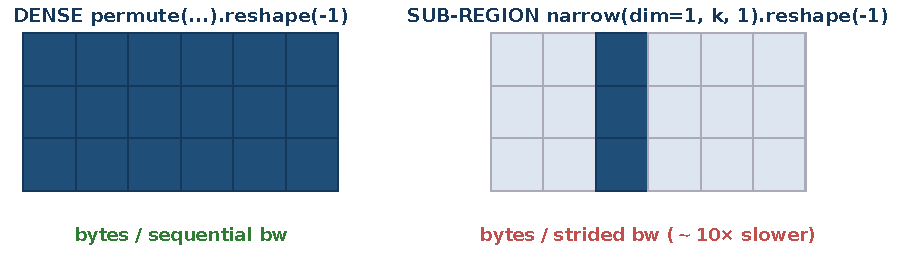
\includegraphics[width=0.78\linewidth]{figures/contiguity.pdf}
\caption{Contiguity-sensitive implicit copies. The same Python
\texttt{...reshape(-1)} is free on a dense permuted source (left,
sequential bw) but pays an $O(\text{numel})$ strided copy on a
sub-region narrow source (right, $4\times$--$10\times$ slower).}
\label{fig:contiguity}
\end{figure}

\paragraph{Side-by-side code: baseline vs agent AllToAllV.}
The agent's deployed AllToAllV runtime collapses the baseline's
AG$+$transpose$+$RS chain (two collectives plus a strided
permute/reshape) into a single padded \texttt{all\_gather} with a
metadata-only slice (Figures \ref{fig:a2av-baseline},
\ref{fig:a2av-agent}).

\begin{figure}[!htbp]
\centering
\begin{BVerbatim}[fontsize=\footnotesize]
def baseline_alltoallv(x, send_counts):
    # AG + transpose + RS path (2 collectives)
    cap = max_send_count(send_counts)
    padded = pad_to_cap(x, cap)
    full = xm.all_gather(padded, dim=0)
    full = full.view(ws, ws, cap, D)
    full = full.transpose(0, 1).contiguous()
    y = xm.reduce_scatter(
        xm.REDUCE_SUM, full.view(-1, D),
        scale=1.0, scatter_dim=0,
        shard_count=ws)
    return unpad(y, recv_counts)
\end{BVerbatim}
\caption{Internal-AWS-optimized baseline AllToAllV:
\texttt{all\_gather} + strided \texttt{permute}/\texttt{contiguous}
+ \texttt{reduce\_scatter}.}
\label{fig:a2av-baseline}
\end{figure}

\begin{figure}[!htbp]
\centering
\begin{BVerbatim}[fontsize=\footnotesize]
def agent_alltoallv(x, send_counts):
    # Pack-and-gather: ONE collective, no strided ops.
    cap = max_send_count(send_counts)
    packed = pack_to_dense(x, cap)
    gathered = xm.all_gather(packed, dim=0)
    gathered = gathered.view(ws, ws, cap, D)
    # Incoming slice is contiguous at outer-axis row `rank`:
    # metadata-only view + slice, no permute, no rs.
    return gathered[:, rank].reshape(-1, D)
\end{BVerbatim}
\caption{Agent-emitted AllToAllV (\emph{pack-and-gather}): one
collective, dispatch count halved, no strided
\texttt{permute}/\texttt{contiguous}. The metadata-only
\texttt{view+slice} replaces the chain that costs strided HBM
bandwidth in the baseline.}
\label{fig:a2av-agent}
\end{figure}


